\frame
{
	\frametitle{Problem Formulation}

	\begin{itemize}
	\item<1-> {\bf Input:} fully connected directed acyclic graph $G=(V,E)$ with source $s$ and sink $t$,
		and flow vector $f$.
	\end{itemize}

	\vspace{0.8cm}
	\begin{center}

\begin{tikzpicture}[font=\small,overlay,
mycirclex/.style={draw, circle, minimum size=1.0em, inner sep = 0.2mm}, 
mydiamond/.style={draw, diamond, minimum size=0.78em, inner sep = 0mm}, 
myrectang/.style={draw, rectangle, minimum size=0.60em, inner sep = 0mm}, 
>=stealth]

\definecolor{mygreen}{rgb}{0, 0.7, 0}
\definecolor{myyellow}{rgb}{0.8, 0.6, 0}

\def\colx{black}
\def\cola{red} 
\def\colb{blue}
\def\colc{violet}
\def\cold{cyan} 
\def\cole{myyellow}
\def\colf{brown}


\def\len{2.0cm}

% G1
\begin{scope}[local bounding box=bbox, xshift=-6.0cm]
\path<1-> node[mycirclex] (v1) at (1.0 * \len, 0) {$s$};
\path<1-> node[mycirclex] (v2) at (2.0 * \len, 0) {$a$};
\path<1-> node[mycirclex] (v3) at (3.0 * \len, 0) {$b$};
\path<1-> node[mycirclex] (v4) at (4.0 * \len, 0) {$c$};
\path<1-> node[mycirclex] (v5) at (5.0 * \len, 0) {$t$};

\path<1-> [draw, \colx, ->, line width=0.04cm] (v1) -- (v2);
\path<1-> [draw, \colx, ->, line width=0.04cm] (v2) -- (v3);
\path<1-> [draw, \colx, ->, line width=0.04cm] (v3) -- (v4);
\path<1-> [draw, \colx, ->, line width=0.04cm] (v4) -- (v5);

\path<1-> [draw, \colx, ->, line width=0.04cm, bend left = 40] (v1) to (v3);
\path<1-> [draw, \colx, ->, line width=0.04cm, bend left = 40] (v3) to (v5);
\path<1-> [draw, \colx, ->, line width=0.04cm, bend left = 40] (v2) to (v4);

\path<1-> node at (1.5 * \len, 0.18cm) {$e_1(8)$};
\path<1-> node at (2.5 * \len, 0.18cm) {$e_2(2)$};
\path<1-> node at (3.5 * \len, 0.18cm) {$e_3(4)$};
\path<1-> node at (4.5 * \len, 0.18cm) {$e_4(10)$};

\path<1-> node at (2.0 * \len, 1.0cm) {$e_5(5)$};
\path<1-> node at (3.0 * \len, 1.0cm) {$e_6(6)$};
\path<1-> node at (4.0 * \len, 1.0cm) {$e_7(3)$};

\end{scope}
%\path<1-> [draw, rounded corners] ($(bbox.south west) - (0.00cm, 0.25cm)$) rectangle ($(bbox.north east) + (0.1cm, 0)$);
%\node at ($(bbox.south) - (0.00cm, 0.2cm)$) [label=below:{$G_2 - G_1 = \{c\}$}]{};


\end{tikzpicture}
\end{center}

	\vspace{-0.1cm}

	\begin{displaymath}
	M = \bordermatrix{
		~   & e_1 & e_2 & e_3 & e_4 & e_5 & e_6 & e_7 \cr
		p_1 & 1 & 1 & 1 & 1 & 0 & 0 & 0 \cr
		p_2 & 1 & 1 & 0 & 0 & 0 & 0 & 1 \cr
		p_3 & 1 & 0 & 0 & 1 & 0 & 1 & 0 \cr
		p_4 & 0 & 0 & 1 & 1 & 1 & 0 & 0 \cr
		p_5 & 0 & 0 & 0 & 0 & 1 & 0 & 1 \cr
	}
	\end{displaymath}

	\vspace{0.1cm}

	\begin{itemize}
	\item<1-> {\bf Output:} $P\subset R(M)$ {\bf and} vector $s$
		such that $f = s\cdot P$ and that $|R(P)|$ is minimized.
	\end{itemize}
}

\frame
{
	\frametitle{Facts}
	Let $\Delta = |E| - |V| + 2$. Let $(P^*, s^*)$ be any optimal solution.
	\vspace{0.3cm}
	\begin{itemize}
	\item<1-> {\bf Fact~1:} $rank(M) = \Delta$.
	\vspace{0.3cm}
	\item<1-> {\bf Fact~2:} $rank(P^*) = |R(P^*)|$.
	\vspace{0.3cm}
	\item<1-> {\bf Fact~3:} $|R(P^*)| \le \Delta$.
	\vspace{0.3cm}
	\item<1-> {\bf Fact~4:} If $|R(M)| = \Delta$, then there is a unique feasible solution: $(M, s)$, where
		$s$ is determined by $f = s\cdot M$. {\bf [trivial case]}
	\end{itemize}
	\vspace{1.0cm}
	\begin{center}

\begin{tikzpicture}[font=\small,overlay,
mycirclex/.style={draw, circle, minimum size=1.0em, inner sep = 0.2mm}, 
mydiamond/.style={draw, diamond, minimum size=0.78em, inner sep = 0mm}, 
myrectang/.style={draw, rectangle, minimum size=0.60em, inner sep = 0mm}, 
>=stealth]

\definecolor{mygreen}{rgb}{0, 0.7, 0}
\definecolor{myyellow}{rgb}{0.8, 0.6, 0}

\def\colx{black}
\def\cola{red} 
\def\colb{blue}
\def\colc{violet}
\def\cold{cyan} 
\def\cole{myyellow}
\def\colf{brown}


\def\len{2.0cm}

% G1
\begin{scope}[local bounding box=bbox, xshift=-6.0cm]
\path<1-> node[mycirclex] (v1) at (1.0 * \len, 0) {$s$};
\path<1-> node[mycirclex] (v2) at (2.0 * \len, 0) {$a$};
\path<1-> node[mycirclex] (v3) at (3.0 * \len, 0) {$b$};
\path<1-> node[mycirclex] (v4) at (4.0 * \len, 0) {$c$};
\path<1-> node[mycirclex] (v5) at (5.0 * \len, 0) {$t$};

\path<1-> [draw, \colx, ->, line width=0.04cm] (v1) -- (v2);
\path<1-> [draw, \colx, ->, line width=0.04cm] (v2) -- (v3);
\path<1-> [draw, \colx, ->, line width=0.04cm] (v3) -- (v4);
\path<1-> [draw, \colx, ->, line width=0.04cm] (v4) -- (v5);

\path<1-> [draw, \colx, ->, line width=0.04cm, bend left = 40] (v1) to (v3);
\path<1-> [draw, \colx, ->, line width=0.04cm, bend left = 40] (v2) to (v5);
\path<1-> [draw, \colx, ->, line width=0.04cm, bend left = 40] (v2) to (v4);

\path<1-> node at (1.5 * \len, 0.15cm) {$e_1$};
\path<1-> node at (2.5 * \len, 0.15cm) {$e_2$};
\path<1-> node at (3.5 * \len, 0.15cm) {$e_3$};
\path<1-> node at (4.5 * \len, 0.15cm) {$e_4$};

\path<1-> node at (2.0 * \len, 0.98cm) {$e_5$};
\path<1-> node at (3.0 * \len, 0.97cm) {$e_6$};
\path<1-> node at (3.5 * \len, 1.36cm) {$e_7$};

\end{scope}
%\path<1-> [draw, rounded corners] ($(bbox.south west) - (0.00cm, 0.25cm)$) rectangle ($(bbox.north east) + (0.1cm, 0)$);
%\node at ($(bbox.south) - (0.00cm, 0.2cm)$) [label=below:{$G_2 - G_1 = \{c\}$}]{};


\end{tikzpicture}
\end{center}

	\vspace{-0.1cm}
}


\frame
{
	\frametitle{Facts~(Cont'd)}

	\vspace{0.3cm}
	\begin{itemize}
	\item<1-> {\bf Fact~5:} If $R(M) > \Delta$ and $|R(P^*)| = \Delta$, then the optimal solution is not unique,
		and the greedy algorithm is guaranteed to get one optimal solution. {\bf [easy case]}
	\end{itemize}

	\vspace{0.5cm}
	\begin{center}

\begin{tikzpicture}[font=\small,overlay,
mycirclex/.style={draw, circle, minimum size=1.0em, inner sep = 0.2mm}, 
mydiamond/.style={draw, diamond, minimum size=0.78em, inner sep = 0mm}, 
myrectang/.style={draw, rectangle, minimum size=0.60em, inner sep = 0mm}, 
>=stealth]

\definecolor{mygreen}{rgb}{0, 0.7, 0}
\definecolor{myyellow}{rgb}{0.8, 0.6, 0}

\def\colx{black}
\def\cola{red} 
\def\colb{blue}
\def\colc{violet}
\def\cold{cyan} 
\def\cole{myyellow}
\def\colf{brown}


\def\len{3.5cm}

% G1
\begin{scope}[local bounding box=bbox, xshift=-7.0cm]
\path<1-> node[mycirclex] (v1) at (1.0 * \len, 0) {$s$};
\path<1-> node[mycirclex] (v2) at (2.0 * \len, 0) {$a$};
\path<1-> node[mycirclex] (v3) at (3.0 * \len, 0) {$t$};

\path<1-> [draw, \colx, ->, line width=0.04cm] (v1) -- (v2);
\path<1-> [draw, \colx, ->, line width=0.04cm] (v2) -- (v3);

\path<1-> [draw, \colx, ->, line width=0.04cm, bend left = 40] (v1) to (v2);
\path<1-> [draw, \colx, ->, line width=0.04cm, bend left = 40] (v2) to (v3);

\path<1-> node at (1.5 * \len, 0.15cm) {$e_2(5)$};
\path<1-> node at (2.5 * \len, 0.15cm) {$e_4(8)$};

\path<1-> node at (1.5 * \len, 0.9cm) {$e_1(9)$};
\path<1-> node at (2.5 * \len, 0.9cm) {$e_3(6)$};

\end{scope}
%\path<1-> [draw, rounded corners] ($(bbox.south west) - (0.00cm, 0.25cm)$) rectangle ($(bbox.north east) + (0.1cm, 0)$);
%\node at ($(bbox.south) - (0.00cm, 0.2cm)$) [label=below:{$G_2 - G_1 = \{c\}$}]{};


\end{tikzpicture}
\end{center}


	\vspace{0.4cm}

	\begin{itemize}
	\item<1-> {\bf Fact~6:} $R(M) > \Delta$ and $|R(P^*)| < \Delta$, the optimal solution
		might be unique. {\bf [hard case]} 
	\end{itemize}

	\vspace{0.5cm}
	\begin{center}

\begin{tikzpicture}[font=\small,overlay,
mycirclex/.style={draw, circle, minimum size=1.0em, inner sep = 0.2mm}, 
mydiamond/.style={draw, diamond, minimum size=0.78em, inner sep = 0mm}, 
myrectang/.style={draw, rectangle, minimum size=0.60em, inner sep = 0mm}, 
>=stealth]

\definecolor{mygreen}{rgb}{0, 0.7, 0}
\definecolor{myyellow}{rgb}{0.8, 0.6, 0}

\def\colx{black}
\def\cola{red} 
\def\colb{blue}
\def\colc{violet}
\def\cold{cyan} 
\def\cole{myyellow}
\def\colf{brown}


\def\len{3.5cm}

% G1
\begin{scope}[local bounding box=bbox, xshift=-7.0cm]
\path<1-> node[mycirclex] (v1) at (1.0 * \len, 0) {$s$};
\path<1-> node[mycirclex] (v2) at (2.0 * \len, 0) {$a$};
\path<1-> node[mycirclex] (v3) at (3.0 * \len, 0) {$t$};

\path<1-> [draw, \colx, ->, line width=0.04cm] (v1) -- (v2);
\path<1-> [draw, \colx, ->, line width=0.04cm] (v2) -- (v3);

\path<1-> [draw, \colx, ->, line width=0.04cm, bend left = 40] (v1) to (v2);
\path<1-> [draw, \colx, ->, line width=0.04cm, bend left = 40] (v2) to (v3);

\path<1-> node at (1.5 * \len, 0.15cm) {$e_2(5)$};
\path<1-> node at (2.5 * \len, 0.15cm) {$e_4(9)$};

\path<1-> node at (1.5 * \len, 0.9cm) {$e_1(9)$};
\path<1-> node at (2.5 * \len, 0.9cm) {$e_3(5)$};

\end{scope}
%\path<1-> [draw, rounded corners] ($(bbox.south west) - (0.00cm, 0.25cm)$) rectangle ($(bbox.north east) + (0.1cm, 0)$);
%\node at ($(bbox.south) - (0.00cm, 0.2cm)$) [label=below:{$G_2 - G_1 = \{c\}$}]{};


\end{tikzpicture}
\end{center}

	\vspace{-0.1cm}

}

\frame
{
	\frametitle{Kernel Theorem}
	\begin{itemize}
	\item {\bf Theorem:} there exist $\Delta - |R(P^*)|$ linearly independent
	{\it non-trivial} vectors $q_k$ satisfying $f\cdot q_k = 0$, $1\le k\le \Delta - |R(P^*)|$.
	\end{itemize}

	\vspace{0.6cm}

	\begin{center}

\begin{tikzpicture}[font=\small,overlay,
mycirclex/.style={draw, circle, minimum size=1.0em, inner sep = 0.2mm}, 
mydiamond/.style={draw, diamond, minimum size=0.78em, inner sep = 0mm}, 
myrectang/.style={draw, rectangle, minimum size=0.60em, inner sep = 0mm}, 
>=stealth]

\definecolor{mygreen}{rgb}{0, 0.7, 0}
\definecolor{myyellow}{rgb}{0.8, 0.6, 0}

\def\colx{black}
\def\cola{red} 
\def\colb{blue}
\def\colc{violet}
\def\cold{cyan} 
\def\cole{myyellow}
\def\colf{brown}


\def\len{3.0cm}

% G1
\begin{scope}[local bounding box=bbox, xshift=-8.0cm]
\path<1-> node[mycirclex] (v1) at (1.0 * \len, 0) {$s$};
\path<1-> node[mycirclex] (v2) at (2.0 * \len, 0) {$a$};
\path<1-> node[mycirclex] (v3) at (3.0 * \len, 0) {$b$};
\path<1-> node[mycirclex] (v4) at (4.0 * \len, 0) {$t$};

\path<1-> [draw, \colc, ->, line width=0.04cm] (v1) -- (v2);
\path<1-> [draw, \colc, ->, line width=0.10cm, bend left = 40] (v2) to (v3);
\path<1-> [draw, \colc, ->, line width=0.10cm, bend left = 40] (v3) to (v4);

\path<1-> [draw, \colb, ->, line width=0.04cm] (v2) -- (v3);
\path<1-> [draw, \colb, ->, line width=0.10cm, bend left = 40] (v1) to (v2);
\path<1-> [draw, \colb, ->, line width=0.04cm, bend left = 40] (v3) to (v4);

\path<1-> [draw, \cola, ->, line width=0.04cm] (v3) -- (v4);
\path<1-> [draw, \cola, ->, line width=0.04cm, bend left = 40] (v1) to (v2);
\path<1-> [draw, \cola, ->, line width=0.04cm, bend left = 40] (v2) to (v3);


%\path<1-> [draw, \colx, ->, line width=0.02cm] (v1) -- (v2);
%\path<1-> [draw, \colx, ->, line width=0.02cm] (v2) -- (v3);
%\path<1-> [draw, \colx, ->, line width=0.02cm] (v3) -- (v4);
%
%\path<1-> [draw, \colx, ->, line width=0.02cm, bend left = 40] (v1) to (v2);
%\path<1-> [draw, \colx, ->, line width=0.02cm, bend left = 40] (v2) to (v3);
%\path<1-> [draw, \colx, ->, line width=0.02cm, bend left = 40] (v3) to (v4);

\path<1-> node at (1.5 * \len, 0.18cm) {$e_2(4)$};
\path<1-> node at (2.5 * \len, 0.18cm) {$e_4(3)$};
\path<1-> node at (3.5 * \len, 0.18cm) {$e_6(2)$};

\path<1-> node at (1.5 * \len, 0.85cm) {$e_1(5)$};
\path<1-> node at (2.5 * \len, 0.85cm) {$e_3(6)$};
\path<1-> node at (3.5 * \len, 0.85cm) {$e_5(7)$};

\end{scope}
%\path<1-> [draw, rounded corners] ($(bbox.south west) - (0.00cm, 0.25cm)$) rectangle ($(bbox.north east) + (0.1cm, 0)$);
%\node at ($(bbox.south) - (0.00cm, 0.2cm)$) [label=below:{$G_2 - G_1 = \{c\}$}]{};


\end{tikzpicture}
\end{center}


	\vspace{-0.5cm}

	\begin{displaymath}
	\bordermatrix{
		~   & e_1 & e_2 & e_3 & e_4 & e_5 & e_6\cr
		p_1 & 1 & 0 & 1 & 0 & 0 & 1 \cr
		p_2 & 1 & 0 & 0 & 1 & 1 & 0 \cr
		p_3 & 0 & 1 & 1 & 0 & 1 & 0 \cr
	} 
	\bordermatrix{
   	   ~& q'_1 & q'_2 & q_1 \cr
		& +1 &  0 & +1  \cr
		& +1 &  0 &  0  \cr
		& -1 & +1 &  0  \cr
		& -1 & +1 & -1  \cr
		&  0 & -1 &  0  \cr
		&  0 & -1 & -1  \cr
	} = 0
	\end{displaymath}

	\begin{itemize}
	\item[1.] Consider the {\bf kernel space} of $P^*$, i.e., $N(P^*) = \{q | P^*\cdot q = 0\}$.
	\item[2.] For any $q\in N(P^*)$, we have $f\cdot q = s\cdot P^* \cdot q = 0$. 
	\item[3.] $\dim(N(P^*)) = |E| - rank(P^*) = |E| - |R(P^*)|$. 
	\item[4.] Non-trivial vectors: $\dim(N(P^*)) - (|V| - 2) = \Delta - |R(P^*)|$. 
	\end{itemize}
}

\frame
{
	\frametitle{Identifying Equations}
	\begin{itemize}
	\item {\bf Conjecture:} $q_i \in \{+1, -1, 0\}$.
	\vspace{0.2cm}
	\item Only consider two simple forms of equations in the current implementation:
		\begin{align}
		f_i & =  f_{i_1} + f_{i_2} + \cdots + f_{i_k} \tag{a}\\
		f_i + f_j & = f_{i_1} + f_{i_2} + \cdots + f_{i_k} \tag{b}
		\end{align}
	\item {\bf Algorithm:} Use the existing pseudo-polynomial-time algorithm for the subset-sum problem.
	\vspace{0.2cm}
	\item For equation of form (a): split $e_i$ into $k$ edges, each with flow
	value of $f_{i_k}$; record these $k$ pairs of edges with equal flow.
	\vspace{0.2cm}
	\item For equation of form (b): use heuristics to split both sides into
			identical set of edges; record these pairs with equal flow.
	\end{itemize}
}

\frame
{
	\frametitle{Merge Adjacent Edges with Equal Flow}
	\vspace{-2.0cm}

	\begin{itemize}
	\item {\bf Algorithm:} merge them directly.
	\end{itemize}

	\vspace{0.8cm}
	\begin{center}

\begin{tikzpicture}[font=\small,overlay,
mycirclex/.style={draw, circle, minimum size=1.0em, inner sep = 0.2mm}, 
mydiamond/.style={draw, diamond, minimum size=0.78em, inner sep = 0mm}, 
myrectang/.style={draw, rectangle, minimum size=0.60em, inner sep = 0mm}, 
>=stealth]

\definecolor{mygreen}{rgb}{0, 0.7, 0}
\definecolor{myyellow}{rgb}{0.8, 0.6, 0}

\def\colx{black}
\def\cola{red} 
\def\colb{blue}
\def\colc{violet}
\def\cold{cyan} 
\def\cole{myyellow}
\def\colf{brown}


\def\len{1.8cm}

% G1
\begin{scope}[local bounding box=bbox, xshift=-6.4cm]
\path<1-> node[mycirclex] (v1) at (1.0 * \len, 0) {$s$};
\path<1-> node[mycirclex] (v2) at (2.0 * \len, 0) {$a$};
\path<1-> node[mycirclex] (v3) at (3.0 * \len, 0) {$b$};
\path<1-> node[mycirclex] (v4) at (4.0 * \len, 0) {$c$};
\path<1-> node[mycirclex] (v5) at (5.0 * \len, 0) {$d$};

\path<1-> [draw, \colx, ->, line width=0.04cm] (v1) -- (v2);
\path<1-> [draw, \colx, ->, line width=0.04cm] (v2) -- (v3);
\path<1-> [draw, \colx, ->, line width=0.04cm] (v3) -- (v4);
\path<1-> [draw, \colx, ->, line width=0.04cm] (v4) -- (v5);

\path<1-> [draw, \colx, ->, line width=0.04cm, bend left = 40] (v1) to (v3);
\path<1-> [draw, \colx, ->, line width=0.04cm, bend left = 27] (v2) to (v5);
\path<1-> [draw, \colx, ->, line width=0.04cm, bend left =-40] (v2) to (v4);

\path<1-> node at (1.5 * \len, 0.18cm) {$e_1$};
\path<1-> node at (2.5 * \len, 0.18cm) {$e_2$};
\path<1-> node at (3.5 * \len, 0.18cm) {$e_3$};
\path<1-> node at (4.5 * \len, 0.18cm) {$e_4$};

\path<1-> node at (2.0 * \len, 0.9cm) {$e_5$};
\path<1-> node at (3.0 * \len,-0.6cm) {$e_6$};
\path<1-> node at (3.5 * \len, 0.9cm) {$e_7$};

\end{scope}
%\path<1-> [draw, rounded corners] ($(bbox.south west) - (0.00cm, 0.25cm)$) rectangle ($(bbox.north east) + (0.1cm, 0)$);
%\node at ($(bbox.south) - (0.00cm, 0.2cm)$) [label=below:{$G_2 - G_1 = \{c\}$}]{};


\end{tikzpicture}
\end{center}


}

\frame
{
	\frametitle{Merge Distant Edges with Equal Flow}
	\vspace{-3.0cm}

	\begin{itemize}
	\item {\bf Algorithm:} {\bf inverse} and {\bf swap} subgraphs based on the its (partial) {\bf nested} structure.
	\end{itemize}

	\vspace{0.8cm}
	\begin{center}

\begin{tikzpicture}[font=\small,overlay,
mycirclex/.style={draw, circle, minimum size=1.0em, inner sep = 0.2mm}, 
mydiamond/.style={draw, diamond, minimum size=0.78em, inner sep = 0mm}, 
myrectang/.style={draw, rectangle, minimum size=0.60em, inner sep = 0mm}, 
>=stealth]

\definecolor{mygreen}{rgb}{0, 0.7, 0}
\definecolor{myyellow}{rgb}{0.8, 0.6, 0}

\def\colx{black}
\def\cola{red} 
\def\colb{blue}
\def\colc{violet}
\def\cold{cyan} 
\def\cole{myyellow}
\def\colf{brown}


\def\len{1.15cm}

% G1
\begin{scope}[local bounding box=bbox, xshift=-3.6cm]
\path<1-> node[mycirclex] (vs) at ( -1 * \len, 0) {$s$};
\path<1-> node[mycirclex] (v0) at (0.0 * \len, 0) {$a$};
\path<1-> node[mycirclex] (v1) at (1.0 * \len, 0) {$b$};
\path<1-> node[mycirclex] (v2) at (2.0 * \len, 0) {$c$};
\path<1-> node[mycirclex] (v3) at (3.0 * \len, 0) {$d$};
\path<1-> node[mycirclex] (v4) at (4.0 * \len, 0) {$e$};
\path<1-> node[mycirclex] (v5) at (5.0 * \len, 0) {$f$};
\path<1-> node[mycirclex] (v6) at (6.0 * \len, 0) {$g$};
\path<1-> node[mycirclex] (v7) at (7.0 * \len, 0) {$t$};

\path<1-> [draw, \colx, ->, line width=0.04cm] (vs) -- (v0);
\path<1-> [draw, \colx, ->, line width=0.04cm] (v0) -- (v1);
\path<1-> [draw, \colx, ->, line width=0.04cm] (v1) -- (v2);
\path<1-> [draw, \colx, ->, line width=0.04cm] (v2) -- (v3);
\path<1-> [draw, \colx, ->, line width=0.04cm] (v3) -- (v4);
\path<1-> [draw, \colx, ->, line width=0.04cm] (v4) -- (v5);
\path<1-> [draw, \colx, ->, line width=0.04cm] (v5) -- (v6);
\path<1-> [draw, \colx, ->, line width=0.04cm] (v6) -- (v7);

\path<1-> [draw, \cola, ->, line width=0.04cm, bend left = 40] (vs) to (v1);
\path<1-> [draw, \colx, ->, line width=0.04cm, bend left = 40] (v0) to (v2);
\path<1-> [draw, \colx, ->, line width=0.04cm, bend left = 40] (v2) to (v4);
\path<1-> [draw, \cola, ->, line width=0.04cm, bend left = 40] (v4) to (v6);
\path<1-> [draw, \colx, ->, line width=0.04cm, bend left = 40] (v5) to (v7);
\path<1-> [draw, \colx, ->, line width=0.04cm, bend left = 40] (v2) to (v7);

\path<1-> node[\colx] at (-.5 * \len, 0.15cm) {$e_1$};
\path<1-> node[\colx] at (0.5 * \len, 0.15cm) {$e_2$};
\path<1-> node[\colx] at (1.5 * \len, 0.15cm) {$e_3$};
\path<1-> node[\colx] at (2.5 * \len, 0.15cm) {$e_4$};
\path<1-> node[\colx] at (3.5 * \len, 0.15cm) {$e_5$};
\path<1-> node[\colx] at (4.5 * \len, 0.15cm) {$e_6$};
\path<1-> node[\colx] at (5.5 * \len, 0.15cm) {$e_7$};
\path<1-> node[\colx] at (6.5 * \len, 0.15cm) {$e_8$};

\path<1-> node[\cola] at (0.0 * \len, 0.65cm) {$e_9$};
\path<1-> node[\colx] at (1.0 * \len, 0.65cm) {$e_{10}$};
\path<1-> node[\colx] at (3.0 * \len, 0.65cm) {$e_{11}$};
\path<1-> node[\cola] at (5.0 * \len, 0.65cm) {$e_{12}$};
\path<1-> node[\colx] at (6.0 * \len, 0.65cm) {$e_{13}$};
\path<1-> node[\colx] at (4.5 * \len, 1.33cm) {$e_{14}$};

\end{scope}
%\path<1-> [draw, rounded corners] ($(bbox.south west) - (0.00cm, 0.25cm)$) rectangle ($(bbox.north east) + (0.1cm, 0)$);
%\node at ($(bbox.south) - (0.00cm, 0.2cm)$) [label=below:{$G_2 - G_1 = \{c\}$}]{};

\path<1-> [draw, line width=0.1cm, ->] (-0.15cm, -0.6cm) -- (-0.15cm, -1.2cm);

% G2
\begin{scope}[local bounding box=bbox, xshift=-3.6cm, yshift=-2.3cm]
\path<1-> node[mycirclex] (vs) at ( -1 * \len, 0) {$s$};
\path<1-> node[mycirclex] (v0) at (0.0 * \len, 0) {$b$};
\path<1-> node[mycirclex] (v1) at (1.0 * \len, 0) {$a$};
\path<1-> node[mycirclex] (v2) at (2.0 * \len, 0) {$c$};
\path<1-> node[mycirclex] (v3) at (3.0 * \len, 0) {$d$};
\path<1-> node[mycirclex] (v4) at (4.0 * \len, 0) {$e$};
\path<1-> node[mycirclex] (v5) at (5.0 * \len, 0) {$f$};
\path<1-> node[mycirclex] (v6) at (6.0 * \len, 0) {$g$};
\path<1-> node[mycirclex] (v7) at (7.0 * \len, 0) {$t$};

\path<1-> [draw, \colx, ->, line width=0.04cm] (vs) -- (v0);
\path<1-> [draw, \colx, ->, line width=0.04cm] (v0) -- (v1);
\path<1-> [draw, \colx, ->, line width=0.04cm] (v1) -- (v2);
\path<1-> [draw, \colx, ->, line width=0.04cm] (v2) -- (v3);
\path<1-> [draw, \colx, ->, line width=0.04cm] (v3) -- (v4);
\path<1-> [draw, \colx, ->, line width=0.04cm] (v4) -- (v5);
\path<1-> [draw, \colx, ->, line width=0.04cm] (v5) -- (v6);
\path<1-> [draw, \colx, ->, line width=0.04cm] (v6) -- (v7);

\path<1-> [draw, \colx, ->, line width=0.04cm, bend left = 40] (vs) to (v1);
\path<1-> [draw, \cola, ->, line width=0.04cm, bend left = 40] (v0) to (v2);
\path<1-> [draw, \colx, ->, line width=0.04cm, bend left = 40] (v2) to (v4);
\path<1-> [draw, \cola, ->, line width=0.04cm, bend left = 40] (v4) to (v6);
\path<1-> [draw, \colx, ->, line width=0.04cm, bend left = 40] (v5) to (v7);
\path<1-> [draw, \colx, ->, line width=0.04cm, bend left = 40] (v2) to (v7);

\path<1-> node[\colx] at (-.5 * \len, 0.15cm) {$e_3$};
\path<1-> node[\colx] at (0.5 * \len, 0.15cm) {$e_2$};
\path<1-> node[\colx] at (1.5 * \len, 0.15cm) {$e_1$};
\path<1-> node[\colx] at (2.5 * \len, 0.15cm) {$e_4$};
\path<1-> node[\colx] at (3.5 * \len, 0.15cm) {$e_5$};
\path<1-> node[\colx] at (4.5 * \len, 0.15cm) {$e_6$};
\path<1-> node[\colx] at (5.5 * \len, 0.15cm) {$e_7$};
\path<1-> node[\colx] at (6.5 * \len, 0.15cm) {$e_8$};

\path<1-> node[\colx] at (0.0 * \len, 0.65cm) {$e_{10}$};
\path<1-> node[\cola] at (1.0 * \len, 0.65cm) {$e_{9}$};
\path<1-> node[\colx] at (3.0 * \len, 0.65cm) {$e_{11}$};
\path<1-> node[\cola] at (5.0 * \len, 0.65cm) {$e_{12}$};
\path<1-> node[\colx] at (6.0 * \len, 0.65cm) {$e_{13}$};
\path<1-> node[\colx] at (4.5 * \len, 1.33cm) {$e_{14}$};

\end{scope}
%\path<1-> [draw, rounded corners] ($(bbox.south west) - (0.00cm, 0.25cm)$) rectangle ($(bbox.north east) + (0.1cm, 0)$);
%\node at ($(bbox.south) - (0.00cm, 0.2cm)$) [label=below:{$G_2 - G_1 = \{c\}$}]{};

\path<1-> [draw, line width=0.1cm, ->] (-0.15cm, -2.9cm) -- (-0.15cm, -3.5cm);

% G3
\begin{scope}[local bounding box=bbox, xshift=-3.6cm, yshift=-4.6cm]
\path<1-> node[mycirclex] (vs) at ( -1 * \len, 0) {$s$};
\path<1-> node[mycirclex] (v0) at (0.0 * \len, 0) {$b$};
\path<1-> node[mycirclex] (v1) at (1.0 * \len, 0) {$a$};
\path<1-> node[mycirclex] (v2) at (2.0 * \len, 0) {$c$};
\path<1-> node[mycirclex] (v3) at (3.0 * \len, 0) {$f$};
\path<1-> node[mycirclex] (v4) at (4.0 * \len, 0) {$g$};
\path<1-> node[mycirclex] (v5) at (5.0 * \len, 0) {$e$};
\path<1-> node[mycirclex] (v6) at (6.0 * \len, 0) {$d$};
\path<1-> node[mycirclex] (v7) at (7.0 * \len, 0) {$t$};

\path<1-> [draw, \colx, ->, line width=0.04cm] (vs) -- (v0);
\path<1-> [draw, \colx, ->, line width=0.04cm] (v0) -- (v1);
\path<1-> [draw, \colx, ->, line width=0.04cm] (v1) -- (v2);
\path<1-> [draw, \colx, ->, line width=0.04cm] (v2) -- (v3);
\path<1-> [draw, \colx, ->, line width=0.04cm] (v3) -- (v4);
\path<1-> [draw, \colx, ->, line width=0.04cm] (v4) -- (v5);
\path<1-> [draw, \colx, ->, line width=0.04cm] (v5) -- (v6);
\path<1-> [draw, \colx, ->, line width=0.04cm] (v6) -- (v7);

\path<1-> [draw, \colx, ->, line width=0.04cm, bend left = 40] (vs) to (v1);
\path<1-> [draw, \cola, ->, line width=0.04cm, bend left = 40] (v0) to (v2);
\path<1-> [draw, \cola, ->, line width=0.04cm, bend left = 40] (v2) to (v4);
\path<1-> [draw, \colx, ->, line width=0.04cm, bend left = 40] (v2) to (v7);
\path<1-> [draw, \colx, ->, line width=0.04cm, bend left = 40] (v3) to (v5);
\path<1-> [draw, \colx, ->, line width=0.04cm, bend left = 40] (v5) to (v7);

\path<1-> node[\colx] at (-.5 * \len, 0.15cm) {$e_3$};
\path<1-> node[\colx] at (0.5 * \len, 0.15cm) {$e_2$};
\path<1-> node[\colx] at (1.5 * \len, 0.15cm) {$e_1$};
\path<1-> node[\colx] at (2.5 * \len, 0.15cm) {$e_6$};
\path<1-> node[\colx] at (3.5 * \len, 0.15cm) {$e_7$};
\path<1-> node[\colx] at (4.5 * \len, 0.15cm) {$e_8$};
\path<1-> node[\colx] at (5.5 * \len, 0.15cm) {$e_4$};
\path<1-> node[\colx] at (6.5 * \len, 0.15cm) {$e_5$};

\path<1-> node[\colx] at (0.0 * \len, 0.65cm) {$e_{10}$};
\path<1-> node[\cola] at (1.0 * \len, 0.65cm) {$e_{9}$};
\path<1-> node[\cola] at (3.0 * \len, 0.65cm) {$e_{12}$};
\path<1-> node[\colx] at (4.0 * \len, 0.65cm) {$e_{13}$};
\path<1-> node[\colx] at (6.0 * \len, 0.65cm) {$e_{11}$};
\path<1-> node[\colx] at (4.5 * \len, 1.33cm) {$e_{14}$};

\end{scope}
%\path<1-> [draw, rounded corners] ($(bbox.south west) - (0.00cm, 0.25cm)$) rectangle ($(bbox.north east) + (0.1cm, 0)$);
%\node at ($(bbox.south) - (0.00cm, 0.2cm)$) [label=below:{$G_2 - G_1 = \{c\}$}]{};



\end{tikzpicture}
\end{center}


}

\frame
{
	\frametitle{Algorithm}
	\begin{itemize}
	\item[1.] Iterate until no change is made to the splice graph. {\bf [core]}
		\vspace{0.2cm}
		\begin{itemize}
		\item[a.] Decompose trivial vertices
		\vspace{0.2cm}
		\item[b.] Identify type~(a) equation and split it
		\vspace{0.2cm}
		\item[c.] Merge equal edges that can be made adjacent
		\vspace{0.2cm}
		\item[d.] Merge equal edges that can not be made adjacent~(*)
		\vspace{0.2cm}
		\item[e.] Identify type~(b) equation and split it~(*)
		\vspace{0.2cm}
		\end{itemize}
	\item[2.] Arbitrarily decompose the remaining splice graph~(easy case, the optimal
			solution is not unique) using greedy algorithm.

	\vspace{0.2cm}
	\item[0.] For real situations that the estimated flow values are not perfect, 
		we can use LP to correct the flow values when identifying equations.

	\end{itemize}
}

\frame
{
	\frametitle{Simulation Results}

	\begin{itemize}
	\item Use iGenome annotation~(gtf file) of Human genome.
	\item Use Flux Simulator to only simulate expression.
	\item Average over 100 independent 100 instances.
	\end{itemize}

	\vspace{0.2cm}
	\def\SA{\hspace*{0pt}}
	\def\SC{\hspace*{-2pt}}
	\def\SB{\hspace*{1pt}}
	\def\SD{\hspace*{3pt}}

	\begin{table}
	\begin{center}%
		\setlength{\tabcolsep}{6.47pt}%
		\begin{tabular}{rrrrrrrrrrrrrrrrrrrrrrrrrrr}%
		\hline
		     & genes & trivial & easy & hard & greedy & scallop \\
		\hline
		average & 11374 & 8203 & 129 & 3036 & 99.3 & {\bf 7.8} \\
		\hline
		ratio(\%)  & 100 & 72.2  & 1.1 & 26.7 & 3.3 & {\bf 0.26} \\
		\hline
		\end{tabular}%
	\end{center}%
	\caption{Capability of returning minimized number of paths.}
	\end{table}

	\vspace{-0.2cm}
	\begin{table}
	\begin{center}%
		\setlength{\tabcolsep}{2.8pt}%
		\begin{tabular}{rrrrrrrrrrrrrrrrrrrrrrrrrrr}%
		\hline
		\multirow{2}{*}{algorithm} &\SB& \multicolumn{3}{c}{gene-level} &\SD& \multicolumn{3}{c}{transcript-level}\\
		\cline{3-5} \cline{7-9}
		     && correct & predicted & ratio && correct & predicted & ratio\\
		\hline
		core    && 2623 & 2725 & 95.6 && 6763 & 7029 & {\bf 96.2} \\
		scallop && 2683 & 3035 & 88.4 && 7608 & 8924 & 85.2 \\
		greedy  && 2617 & 3035 & 86.2 && 7304 & 9037 & 80.8 \\
		\hline
		\end{tabular}%
	\end{center}%
	\caption{Accuracy of predicted transcripts.}
	\end{table}

}

\frame
{
	\frametitle{Next Steps}

	\begin{itemize}
	\item[1.] Prove/disprove the conjecture.
	\vspace{0.3cm}
	\item[2.] Work on generating high quality splice graph~(identify exons and estimate
			flow values) from sequence data.
	\vspace{0.3cm}
	\item[3.] Design better algorithms to use type (b) and even more complicated equations.
	\vspace{0.3cm}
	\item[4.] Identify additional biological information to select the correct one from 
		multiple optimal solutions.
	\vspace{0.3cm}
	\item[5.] Think about applying this algorithm to other problems, for example, to
		help the EM-step of the quantification algorithm.
	\end{itemize}
}

\frame
{
	\frametitle{Building Nested Graph}
	\vspace{-1.2cm}

	\begin{itemize}
	\item {\bf Problem:} given splice graph $G=(V,E)$, to build $G'=(V,E')$.
	\item For $u,v\in V$, define subgraph $G_{uv} = (V_{uv}, E_{uv})$:
	$V_{uv}$ is the set of vertices that can be reached from $u$ and can reach $t$; $E_{uv}$ 
	is the set of edges for each of which both ends are in $V_{uv}$.
	\item $G_{uv}$ is {\bf independent} if for each $w\in V_{uv}\setminus \{u,v\}$, all adjacent edges
	of $w$ are in $E_{uv}$.  $E' = \{(u,v) | G_{uv} \textrm{ is independent}\}$.
	\item We can prove that $G'$ is a nested graph.
	\end{itemize}
	\vspace{0.8cm}
	\begin{center}

\begin{tikzpicture}[font=\small,overlay,
mycirclex/.style={draw, circle, minimum size=1.0em, inner sep = 0.2mm}, 
mydiamond/.style={draw, diamond, minimum size=0.78em, inner sep = 0mm}, 
myrectang/.style={draw, rectangle, minimum size=0.60em, inner sep = 0mm}, 
>=stealth]

\definecolor{mygreen}{rgb}{0, 0.7, 0}
\definecolor{myyellow}{rgb}{0.8, 0.6, 0}

\def\colx{black}
\def\cola{red} 
\def\colb{blue}
\def\colc{violet}
\def\cold{cyan} 
\def\cole{myyellow}
\def\colf{brown}


\def\len{1.15cm}


% G1
\begin{scope}[local bounding box=bbox, xshift=-3.6cm]
\path<1-> node[mycirclex] (vs) at ( -1 * \len, 0) {$s$};
\path<1-> node[mycirclex] (v0) at (0.0 * \len, 0) {$a$};
\path<1-> node[mycirclex] (v1) at (1.0 * \len, 0) {$b$};
\path<1-> node[mycirclex] (v2) at (2.0 * \len, 0) {$c$};
\path<1-> node[mycirclex] (v3) at (3.0 * \len, 0) {$d$};
\path<1-> node[mycirclex] (v4) at (4.0 * \len, 0) {$e$};
\path<1-> node[mycirclex] (v5) at (5.0 * \len, 0) {$f$};
\path<1-> node[mycirclex] (v6) at (6.0 * \len, 0) {$g$};
\path<1-> node[mycirclex] (v7) at (7.0 * \len, 0) {$t$};

\path<1-> [draw, \colx, ->, line width=0.04cm] (vs) -- (v0);
\path<1-> [draw, \colx, ->, line width=0.04cm] (v0) -- (v1);
\path<1-> [draw, \colx, ->, line width=0.04cm] (v1) -- (v2);
\path<1-> [draw, \colx, ->, line width=0.04cm] (v2) -- (v3);
\path<1-> [draw, \colx, ->, line width=0.04cm] (v3) -- (v4);
\path<1-> [draw, \colx, ->, line width=0.04cm] (v4) -- (v5);
\path<1-> [draw, \colx, ->, line width=0.04cm] (v5) -- (v6);
\path<1-> [draw, \colx, ->, line width=0.04cm] (v6) -- (v7);

\path<1-> [draw, \colx, ->, line width=0.04cm, bend left = 40] (vs) to (v1);
\path<1-> [draw, \colx, ->, line width=0.04cm, bend left = 40] (v0) to (v2);
\path<1-> [draw, \colx, ->, line width=0.04cm, bend left = 40] (v2) to (v4);
\path<1-> [draw, \colx, ->, line width=0.04cm, bend left = 40] (v4) to (v6);
\path<1-> [draw, \colx, ->, line width=0.04cm, bend left = 40] (v5) to (v7);
\path<1-> [draw, \colx, ->, line width=0.04cm, bend left = 40] (v2) to (v7);

\path<1-> node[\colx] at (-.5 * \len, 0.15cm) {$e_1$};
\path<1-> node[\colx] at (0.5 * \len, 0.15cm) {$e_2$};
\path<1-> node[\colx] at (1.5 * \len, 0.15cm) {$e_3$};
\path<1-> node[\colx] at (2.5 * \len, 0.15cm) {$e_4$};
\path<1-> node[\colx] at (3.5 * \len, 0.15cm) {$e_5$};
\path<1-> node[\colx] at (4.5 * \len, 0.15cm) {$e_6$};
\path<1-> node[\colx] at (5.5 * \len, 0.15cm) {$e_7$};
\path<1-> node[\colx] at (6.5 * \len, 0.15cm) {$e_8$};

\path<1-> node[\colx] at (0.0 * \len, 0.65cm) {$e_9$};
\path<1-> node[\colx] at (1.0 * \len, 0.65cm) {$e_{10}$};
\path<1-> node[\colx] at (3.0 * \len, 0.65cm) {$e_{11}$};
\path<1-> node[\colx] at (5.0 * \len, 0.65cm) {$e_{12}$};
\path<1-> node[\colx] at (6.0 * \len, 0.65cm) {$e_{13}$};
\path<1-> node[\colx] at (4.5 * \len, 1.30cm) {$e_{14}$};

\end{scope}
%\path<1-> [draw, rounded corners] ($(bbox.south west) - (0.00cm, 0.25cm)$) rectangle ($(bbox.north east) + (0.1cm, 0)$);
%\node at ($(bbox.south) - (0.00cm, 0.2cm)$) [label=below:{$G_2 - G_1 = \{c\}$}]{};

\path<1-> [draw, line width=0.1cm, ->] (-0.15cm, -0.4cm) -- (-0.15cm, -1.0cm);

% G2
\begin{scope}[local bounding box=bbox, xshift=-3.6cm, yshift=-2.0cm]
\path<1-> node[mycirclex] (vs) at ( -1 * \len, 0) {$s$};
\path<1-> node[mycirclex] (v0) at (0.0 * \len, 0) {$a$};
\path<1-> node[mycirclex] (v1) at (1.0 * \len, 0) {$b$};
\path<1-> node[mycirclex] (v2) at (2.0 * \len, 0) {$c$};
\path<1-> node[mycirclex] (v3) at (3.0 * \len, 0) {$d$};
\path<1-> node[mycirclex] (v4) at (4.0 * \len, 0) {$e$};
\path<1-> node[mycirclex] (v5) at (5.0 * \len, 0) {$f$};
\path<1-> node[mycirclex] (v6) at (6.0 * \len, 0) {$g$};
\path<1-> node[mycirclex] (v7) at (7.0 * \len, 0) {$t$};

\path<1-> [draw, \colx, ->, line width=0.04cm] (vs) -- (v0);
\path<1-> [draw, \colx, ->, line width=0.04cm] (v0) -- (v1);
\path<1-> [draw, \colx, ->, line width=0.04cm] (v1) -- (v2);
\path<1-> [draw, \colx, ->, line width=0.04cm] (v2) -- (v3);
\path<1-> [draw, \colx, ->, line width=0.04cm] (v3) -- (v4);
\path<1-> [draw, \colx, ->, line width=0.04cm] (v4) -- (v5);
\path<1-> [draw, \colx, ->, line width=0.04cm] (v5) -- (v6);
\path<1-> [draw, \colx, ->, line width=0.04cm] (v6) -- (v7);

\path<1-> [draw, \colx, ->, line width=0.04cm, bend left = 40] (vs) to (v2);
\path<1-> [draw, \colx, ->, line width=0.04cm, bend left = 40] (v2) to (v4);
\path<1-> [draw, \colx, ->, line width=0.04cm, bend left = 40] (v4) to (v7);
\path<1-> [draw, \colx, ->, line width=0.04cm, bend left = 40] (v2) to (v7);

\path<1-> node[\colx] at (-.5 * \len, 0.15cm) {$e_1$};
\path<1-> node[\colx] at (0.5 * \len, 0.15cm) {$e_2$};
\path<1-> node[\colx] at (1.5 * \len, 0.15cm) {$e_3$};
\path<1-> node[\colx] at (2.5 * \len, 0.15cm) {$e_4$};
\path<1-> node[\colx] at (3.5 * \len, 0.15cm) {$e_5$};
\path<1-> node[\colx] at (4.5 * \len, 0.15cm) {$e_6$};
\path<1-> node[\colx] at (5.5 * \len, 0.15cm) {$e_7$};
\path<1-> node[\colx] at (6.5 * \len, 0.15cm) {$e_8$};

\path<1-> node[\colx] at (0.5 * \len, 0.88cm) {$e_{15}$};
\path<1-> node[\colx] at (3.0 * \len, 0.65cm) {$e_{11}$};
\path<1-> node[\colx] at (5.5 * \len, 0.88cm) {$e_{16}$};
\path<1-> node[\colx] at (4.5 * \len, 1.30cm) {$e_{14}$};

\end{scope}
%\path<1-> [draw, rounded corners] ($(bbox.south west) - (0.00cm, 0.25cm)$) rectangle ($(bbox.north east) + (0.1cm, 0)$);
%\node at ($(bbox.south) - (0.00cm, 0.2cm)$) [label=below:{$G_2 - G_1 = \{c\}$}]{};


\end{tikzpicture}
\end{center}

}

\frame
{
	\frametitle{Merge Two Edges}

	\vspace{1.0cm}
	\begin{center}

\begin{tikzpicture}[font=\small,overlay,
mycirclex/.style={draw, circle, minimum size=1.0em, inner sep = 0.2mm}, 
mydiamond/.style={draw, diamond, minimum size=0.78em, inner sep = 0mm}, 
myrectang/.style={draw, rectangle, minimum size=0.60em, inner sep = 0mm}, 
>=stealth]

\definecolor{mygreen}{rgb}{0, 0.7, 0}
\definecolor{myyellow}{rgb}{0.8, 0.6, 0}

\def\colx{black}
\def\cola{red} 
\def\colb{blue}
\def\colc{violet}
\def\cold{cyan} 
\def\cole{myyellow}
\def\colf{brown}


\def\len{1.8cm}

% G1
\begin{scope}[local bounding box=bbox, xshift=-6.4cm, yscale=1.2]
\path<2-> node[mycirclex] (v1) at (1.0 * \len, 0) {$s$};
\path<2-> node[mycirclex] (v2) at (2.0 * \len, 0) {$a$};
\path<2-> node[mycirclex] (v3) at (3.0 * \len, 0) {$b$};
\path<2-> node[mycirclex] (v4) at (4.0 * \len, 0) {$c$};
\path<2-> node[mycirclex] (v5) at (5.0 * \len, 0) {$d$};
\path<2-> node[mycirclex] (v6) at (6.0 * \len, 0) {$t$};

\path<2-> [draw, \colb, ->, line width=0.10cm] (v1) -- (v2);
\path<2-> [draw, \colb, ->, line width=0.10cm] (v3) -- (v4);
\path<2-> [draw, \colb, ->, line width=0.10cm] (v5) -- (v6);
\path<2-> [draw, \colb, ->, line width=0.10cm, bend left = 30] (v2) to (v3);
\path<2-> [draw, \colb, ->, line width=0.10cm, bend left = 30] (v4) to (v5);

\path<2-> [draw, \cola, ->, line width=0.05cm] (v1) -- (v2);
\path<2-> [draw, \cola, ->, line width=0.05cm] (v2) -- (v3);
\path<2-> [draw, \cola, ->, line width=0.05cm] (v3) -- (v4);
\path<2-> [draw, \cola, ->, line width=0.05cm] (v4) -- (v5);
\path<2-> [draw, \cola, ->, line width=0.05cm] (v5) -- (v6);

\path<3-> [draw, line width = 0.08cm, <->] (3.5 * \len, -0.4cm) to node[label=right:{$P_1 + P_2 = P_1' + P_2'$}]{} (3.5 * \len, -1.5cm);
\end{scope}

% G2
\begin{scope}[local bounding box=bbox, xshift=-6.4cm, yscale=1.2, yshift = -2.0cm]
\path<3-> node[mycirclex] (v1) at (1.0 * \len, 0) {$s$};
\path<3-> node[mycirclex] (v2) at (2.0 * \len, 0) {$a$};
\path<3-> node[mycirclex] (v3) at (3.0 * \len, 0) {$b$};
\path<3-> node[mycirclex] (v4) at (4.0 * \len, 0) {$c$};
\path<3-> node[mycirclex] (v5) at (5.0 * \len, 0) {$d$};
\path<3-> node[mycirclex] (v6) at (6.0 * \len, 0) {$t$};

\path<3-> [draw, \colb, ->, line width=0.10cm] (v1) -- (v2);
\path<3-> [draw, \colb, ->, line width=0.10cm] (v3) -- (v4);
\path<3-> [draw, \colb, ->, line width=0.10cm] (v5) -- (v6);
\path<3-> [draw, \colb, ->, line width=0.10cm, bend left = 30] (v2) to (v3);
\path<3-> [draw, \cola, ->, line width=0.05cm, bend left = 30] (v4) to (v5);

\path<3-> [draw, \cola, ->, line width=0.05cm] (v1) -- (v2);
\path<3-> [draw, \cola, ->, line width=0.05cm] (v2) -- (v3);
\path<3-> [draw, \cola, ->, line width=0.05cm] (v3) -- (v4);
\path<3-> [draw, \colb, ->, line width=0.10cm] (v4) -- (v5);
\path<3-> [draw, \cola, ->, line width=0.05cm] (v5) -- (v6);

\end{scope}



\end{tikzpicture}
\end{center}


	\vspace{2.0cm}
	\begin{itemize}
	\item If $e_x$ and $e_y$ intersect, then they cannot be merged.
	\item Otherwise, after adding $e_x$ and $e_y$ to $G'$, $G'$ is still nested.
	\item {\bf Algorithm:} dynamic programming: for each interval, determine
	whether $e_x$ and $e_y$ can be moved to its left boundary and right boundary.
		\begin{itemize}
		\item Original edges in $G'$ can be used to {\bf inverse}.
		\item Subset of adjacent original edges in $G'$ can be used to {\bf swap}.
		\end{itemize}
	\end{itemize}
}
